\section{Populations and samples}
\subsection{Definitions}
\begin{description}
    \item[Population] The whole set of items that are of interest
    \item[Census] Observes or measures every member of a population
    \item[Sample] A selection of observations taken from a subset of the population which is used
    \item[Sampling unit] Individual units of a population that cam be sampled
    \item[Sampling frame] A list of all people or item that can potentially be involved in the sample
\end{description}

\subsection{Census}
\subsubsection{Advantages}
\begin{itemize}
    \item Gives a completely accurate result, no bias
\end{itemize}
\subsubsection{Disadvantages}
\begin{itemize}
    \item Time consuming and expensive
    \item Cannot be used when the testing process destroys the item
    \item Hard to process large quantity of data
\end{itemize}
\subsection{Sample}
\subsubsection{Advantages}
\begin{itemize}
    \item Easier to implement
    \item Quicker to implement
    \item Less data to process
    \item Cheaper to implement
\end{itemize}
\subsubsection{Disadvantages}
\begin{itemize}
    \item The data may not be representative
    \item The sample may not be large enough to give information about small sub-groups of the population
\end{itemize}
\subsection{Sample size}
\begin{itemize}
    \item Larger sample size = better accuracy
    \item If the population is varied a larger sample size is needed to make sure that the sample is representative
\end{itemize}


\section{Random sampling methods}
\subsection{Simple random sampling}
\subsubsection{Definition}
\begin{itemize}
    \item Every possible sample of size $n$ has an \textbf{equal chance} of being picked
\end{itemize}
\subsubsection{Method}
\begin{enumerate}
    \item Each sampling unit is numbered from 1 to $n$
    \item Generate $x$ random number between 1 to $n$ using random number generators / lottery picks / random number tables (or draw out $x$ names from the lottery hat), ignoring repeats
    \item Sampling units corresponding to these numbers become the sample
    \item Data taken from the sample
\end{enumerate}
\subsubsection{Advantages}
\begin{itemize}
    \item Free of bias
    \item Easy and cheap to implement for small populations and small samples
    \item Each sampling unit has a known and equal chance of selection
\end{itemize}
\subsubsection{Disadvantages}
\begin{itemize}
    \item Not suitable when the population size or the sample size is large as it is potentially time consuming, disruptive and expensive
    \item A sampling frame is needed
    \item Chance of being unrepresentative
\end{itemize}
\subsection{Systematic sampling}
\subsubsection{Definition}
\begin{itemize}
    \item The required elements are chosen at \textbf{regular intervals} from an \textbf{ordered list}
\end{itemize}
\subsubsection{Method}
\begin{enumerate}
    \item The population is ordered with a unique number each from 1 to $n$
    \item Required elements are chosen at regular intervals i.e. take every $k$th elements where $k=\frac{\text{Population size}}{\text{Sample size}}$
    \item Starting at random item between 1 and $k$ using a random number generator
    \item Take that item and select the remaining data at the chosen interval
    \item[*] \textbf{Show working}
\end{enumerate}
\subsubsection{Advantages}
\begin{itemize}
    \item Simple and quick to use
    \item Suitable for large samples and large populations
\end{itemize}
\subsubsection{Disadvantages}
\begin{itemize}
    \item A sampling frame is needed
    \item It can introduce bias if the sampling frame is not random
\end{itemize}
\subsection{Stratified sampling}
\subsubsection{Definition}
\begin{itemize}
    \item The population is divided into mutually exclusive strata and a random sample is taken from each
\end{itemize}
\subsubsection{Method}
\begin{enumerate}
    \item Population divided into \textbf{non-overlapping} groups / strata
    \item Same proportion ($\frac{\text{Sample size}}{\text{Population size}}$) sampled from each strata (\textbf{show working} for the total population and the size of each strata individually, round if needed)
    \item Simple random sampling carried out in each group (explain in more details here)
\end{enumerate}
\subsubsection{Advantages}
\begin{itemize}
    \item Sample accurately reflects the population structure
    \item Guarantees proportional representation of groups within a population
\end{itemize}
\subsubsection{Disadvantages}
\begin{itemize}
    \item Population must be clearly classified into distinct strata
    \item Selection within each stratum suffers from the same disadvantages as simple random sampling
\end{itemize}
\section{Non-random sampling methods}
\subsection{Quota sampling}
\subsubsection{Method}
\begin{enumerate}
    \item Population divided into groups according to a given characteristic
    \item A quota group is set to try and reflect the group's proportion in the whole population
    \item An interviewer or researcher selects a sample that reflects the characteristics of the whole population (opportunity sampling)
    \item[*] \textbf{Show working}
\end{enumerate}
\subsubsection{Advantages}
\begin{itemize}
    \item Allows a small sample to still be representative of the population
    \item No sampling frame required
    \item Quick, easy, inexpensive
    \item Allows for easy comparison between different groups of population
\end{itemize}
\subsubsection{Disadvantages}
\begin{itemize}
    \item Non-random sampling can introduce bias
    \item Population must be divided into groups, which can be costly or inaccurate
    \item Increasing scope of study increases number of groups, adding time or expense
    \item Non-responses are not recorded
\end{itemize}

\subsection{Opportunity / convenience / pragmatic sampling}
\subsubsection{Method}
\begin{enumerate}
    \item Sample taken from people who are available at time of study and meet the criteria
\end{enumerate}
\subsubsection{Advantages}
\begin{itemize}
    \item Easy to carry out
    \item No sampling frame required
    \item Inexpensive
\end{itemize}
\subsubsection{Disadvantages}
\begin{itemize}
    \item Likely to be unrepresentative
    \item Highly dependent on individual researcher (likely to be biased)
\end{itemize}

\section{Large data set}
\subsection{Scope}
\begin{itemize}
    \item Months included: May - October
    \item Years included: 2015 and 1987
\end{itemize}
\subsection{Background information}
%\subsection{Cities}
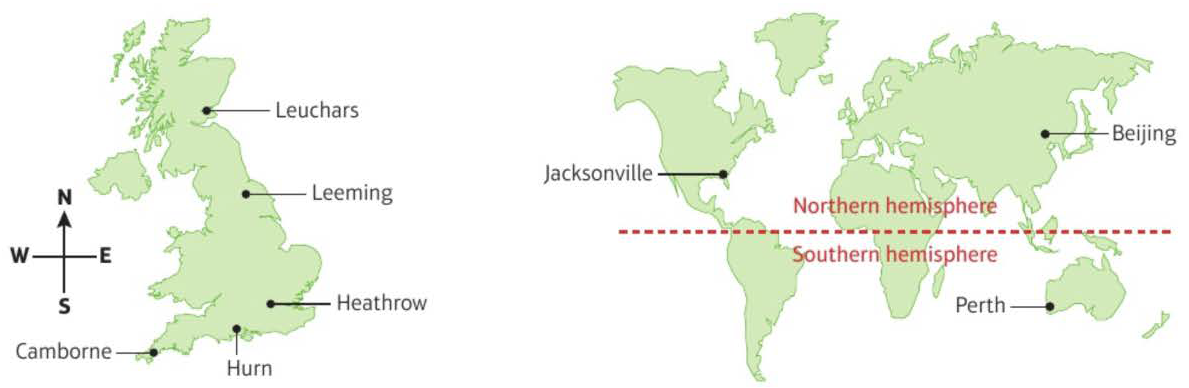
\includegraphics{LDSmap}\\
\begin{tabular}{|p{2cm}|p{15cm}|}
    \hline
    \textbf{City} & \textbf{Climate and geographical locations}                                                                                                           \\
    \hline
    Leuchars      & Coastal \newline NE of Scotland \newline Climate generally warm and temperate \newline significant rainfall throughout the year                       \\
    \hline
    Leeming       & \textbf{Inland} \newline Climate generally warm and temperate \newline significant rainfall throughout the year                                       \\
    \hline
    Heathrow      & \textbf{Inland} \newline Temperate oceanic climate \newline Cool to warm summers \newline cold winters                                                \\
    \hline
    Hurn          & Coastal \newline Southern England \newline Mild climate \newline Warm summers + \textbf{heavy rainfall} often in \textbf{mild} winters                \\
    \hline
    Camborne      & Coastal \newline Cornwall (SW England) \newline Climate generally warm and temperate \newline \textbf{High rainfall} even in driest months            \\
    \hline
    Beijing       & \textbf{Inland} (150km from the sea) \newline Northern hemisphere but relatively far South, so it tends to be \textbf{hot and humid} in summer months \\
    \hline
    Jacksonville  & Coastal \newline Northern hemisphere but relatively far South, so it tends to be \textbf{hot and humid} in summer months                              \\
    \hline
    Perth         & Coastal \newline In the \textbf{southern hemisphere} - in winter during May - Oct                                                                     \\
    \hline
\end{tabular}\\
(Cities are ordered from North to South)

%\subsection{Weather incidents}
\begin{description}
    \item[1987] ``Great storm" in UK in October so there are unusually high winds, mild ``El Nino" impact globally
    \item[2015] Strong ``El Nino" impact espacially in the US so there is cooler temperature and higher rainfall
\end{description}

\subsection{Data recorded}
%\subsection{Definitions}
\begin{tabular}{|p{5.5cm}|p{11.5cm}|}
    \hline
    \textbf{Variable}               & \textbf{Unit}                                                                                                                                                                                                      \\
    \hline
    Daily mean temperature          & The average of the hourly temperature (\textcelsius) readings, 09:00 – 09:00 GMT \newline A reading which is not available is listed as ‘n/a’.
    \\
    \hline
    Daily total rainfall            & Daily total precipitation (mm) 09:00 – 09:00 GMT
    (includes snow or hail, which is melted and measured in the same way as rainfall.) \newline
    'Trace' (tr) is less than 0.05 mm. \newline A reading which is not available will be shown by ‘n/a’
    \\
    \hline
    Daily total sunshine            & Sunshine amounts are recorded in hours and tenths and show the amount of bright sunshine recorded on the day of entry. \newline A reading which is not available will be shown by ‘n/a’                            \\
    \hline
    Daily maximum relative humidity & A measure of how close the air is to being saturated with water vapour. \newline Relative humidities above 95\% are associated with mist and fog. \newline A reading which is not available will be shown by ‘n/a’
    \\
    \hline
    Daily mean wind direction       & The daily mean wind direction the wind is \textbf{coming from}, (clockwise from North) is averaged and rounded to the nearest 10\textdegree \newline
    Readings which are not available are listed as ‘n/a’.
    \\
    \hline
    Daily mean windspeed            & Daily average windspeed \newline Readings are taken 00:00 – 00:00 GMT, in knots (kn, 1 knot = 1.15mph) \newline
    Readings which are not available are listed as ‘n/a’.                                                                                                                                                                                                \\
    \hline
    Daily maximum gust              & Maximum instantaneous wind speed \newline Readings are taken 00:00 – 00:00 GMT, in knots (kn, 1 knot = 1.15mph) \newline
    Readings which are not available are listed as ‘n/a’.                                                                                                                                                                                                \\
    \hline
    Daily maximum gust direction    & The direction from which the wind was blowing when the maximum gust during the hour commencing at the time of entry occurred, and is measured in degrees from true north.  \newline
    Readings which are not available are listed as ‘n/a’.                                                                                                                                                                                                \\
    \hline
    Daily mean cloud cover          & Measured in eights (oktas)                                                                                                                                                                                         \\
    \hline
    Daily mean visibility           & The greatest distance at which an object can be seen and recognized in daylight, or at night could be seen and recognized if the general illumination were raised to daylight level.
    \newline Visibility is measured horizontally, in decametres (Dm) dam = 10m \newline A dash (-) indicates data not available.
    \\
    \hline
    Daily mean pressure             & Mean sea level pressure, calculated from a measurement made at station level. \newline Measured in hectopascals (hPa) 	where 1 hPa = 1 millibar
    \\
    \hline
\end{tabular}
\subsection{Unit and precision of data}
\begin{tabular}{|l|l|l|}
    \hline
    \textbf{Variable}               & \textbf{Unit}               & \textbf{Precision}                           \\
    \hline
    Daily mean temperature          & \textcelsius                & to 1 dp                                      \\
    \hline
    Daily total rainfall            & mm                          & to 1 dp (tr = less than 0.05 mm, treat as 0) \\
    \hline
    Daily total sunshine            & hours                       & to 1 dp                                      \\
    \hline
    Daily maximum relative humidity & as a percentage             & nearest integer                              \\
    \hline
    Daily mean wind direction       & degree + cardinal direction & nearest integer                              \\
    \hline
    Daily mean windspeed            & knots / Beaufort conversion & nearest integer                              \\
    \hline
    Daily maximum gust              & knots                       & nearest integer                              \\
    \hline
    Daily maximum gust direction    & degree + cardinal direction & nearest integer                              \\
    \hline
    Daily mean cloud cover          & oktas                       & integer from 0-8                             \\
    \hline
    Daily mean visibility           & decametres (Dm)             & nearest 100                                  \\
    \hline
    Daily mean pressure             & hectopascals (hPa)          & nearest integer                              \\
    \hline
\end{tabular}
%* Wind direction is defined as the direction where the wind \textbf{comes from}

\subsection{Typical values}
\subsubsection{Temperature and wind speed}
\begin{tabular}{|l|l|l|}
    \hline
    \textbf{Location} & \textbf{Temperature range (\textcelsius)} & \textbf{Wind speed range (knots)} \\
    \hline
    Leuchars          & 4-19                                      & 3-23                              \\
    \hline
    Leeming           & 4-23                                      & 3-17                              \\
    \hline
    Heathrow          & 8-29                                      & 3-19                              \\
    \hline
    Hurn              & 6-24                                      & 2-19                              \\
    \hline
    Camborne          & 10-20                                     & 3-18                              \\
    \hline
    Beijing           & 8-33                                      & 2-9                               \\
    \hline
    Jacksonville      & 15-31                                     & 1-12                              \\
    \hline
    Perth             & 8-25                                      & 4-14                              \\
    \hline
\end{tabular}

\subsubsection{Other data}
\begin{tabular}{|p{4.8cm} | p{12.2cm}|}
    \hline
    \textbf{Variable}            & \textbf{Typical values}                                                  \\
    \hline
    Gust                         & 20 kn                                                                    \\
    \hline
    Rainfall                     & 0-60 mm in the UK, more extreme maximums elsewhere (e.g. 102mm in Perth) \\
    \hline
    Pressure                     & $1013 \pm 25$ Pa                                                         \\
    \hline
    Wind speed on Beaufort Scale & Mostly light / moderate. Maximum is fresh (5)                            \\
    \hline
    Sunshine                     & 0-16 hours                                                               \\
    \hline
    Cloud cover                  & 0-8 oktas                                                                \\
    \hline
\end{tabular}

\subsection{Cleaning data}
\begin{description}
    \item[tr] Needs to be replaced with a number between $0$ and $0.05$ (ideally $0.025$ as it is the midpoint) before processing data
    \item[n/a] Problem = data isn't available, usually ignored when doing calculations
\end{description}